\section{Descripción General}
Diseñar y construir un prototipo de sistema automatizado para la clasificación de mandarinas basado en su grado de madurez, utilizando sensores ópticos que operan bajo principios electromagnéticos para mejorar la eficiencia y objetividad del proceso de selección.

\section{Objetivos Específicos}
\begin{enumerate}
    \item Analizar las propiedades ópticas de las mandarinas para definir un criterio de madurez.
    \item Seleccionar y calibrar los componentes electrónicos (sensores, microcontrolador, actuadores).
    \item Diseñar e implementar una estructura mecánica para el transporte y clasificación.
    \item Desarrollar el software de control que toma las decisiones de clasificación.
    \item Validar el funcionamiento del prototipo integrado con pruebas reales.
\end{enumerate}

\section{Alcance del Proyecto}
Este proyecto busca demostrar, de manera práctica, cómo los principios del electromagnetismo y la visión por computadora pueden aplicarse en un sistema de clasificación de frutas. Para ello, se construyó una banda transportadora de 40 cm equipada con una cámara, una Raspberry Pi y servomotores que permiten identificar y separar mandarinas de acuerdo con su grado de madurez.

El alcance está enfocado en el desarrollo de un prototipo funcional a escala, utilizando materiales accesibles como MDF, motores DC y componentes electrónicos básicos. Con este sistema, se busca simular un proceso real de selección postcosecha, validando que con recursos limitados es posible diseñar soluciones automatizadas que mejoren la eficiencia y objetividad de la clasificación de productos agrícolas.

\section{Limitaciones}
\begin{itemize}
    \item El modelo está pensado para frutas simuladas o de prueba, no para cargas reales de gran tamaño o peso.
    \item El sistema funciona únicamente sobre superficies planas y estables, sin incorporar mecanismos de suspensión ni adaptación a diferentes terrenos.
    \item La automatización es básica: se centra en la detección de color para determinar madurez, sin integrar algoritmos avanzados de visión artificial ni sensores adicionales.
    \item La velocidad de operación es reducida, ya que se priorizó la estabilidad y el control del motor antes que la rapidez del transporte.
\end{itemize}

\section{Estructura del Proyecto}
El prototipo consiste en una banda transportadora de 40 cm de longitud diseñada para clasificar mandarinas simuladas según su grado de madurez.

El proceso de funcionamiento es el siguiente:
\begin{enumerate}
    \item Un motor DC transporta el fruto hasta la zona de análisis.
    \item Una cámara conectada a una Raspberry Pi 4 captura la imagen en tiempo real.
    \item Un programa en Python con la librería OpenCV analiza el color:
    \begin{itemize}
        \item Verde intenso o verde amarillento: fruto inmaduro.
        \item Amarillo o naranja brillante: fruto maduro.
    \end{itemize}
    \item Según la decisión, la Raspberry Pi activa uno de dos servomotores que desvían el fruto hacia el canal correspondiente.
\end{enumerate}

De esta manera, el sistema opera de forma autónoma, replicando un proceso real de selección postcosecha con tecnología accesible y de código abierto.

\begin{figure}[H]
    \centering
    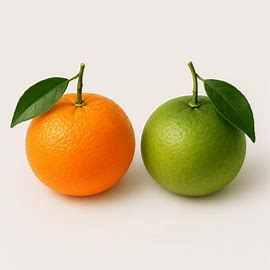
\includegraphics[width=0.7\textwidth]{./assets/mandarinas.jpeg}
    \caption{Mandarinas clasificadas según su grado de madurez en el prototipo.}
    \label{fig:mandarinas}
\end{figure}

\newpage
\section{Materiales y Métodos}

A continuación se detallan los materiales y componentes utilizados en la implementación del sistema de clasificación automática de frutas:

\begin{table}[H]
\centering
\caption{Lista de materiales y componentes del proyecto}
\begin{tabular}{|p{0.35\textwidth}|p{0.6\textwidth}|}
\hline
\textbf{Componente} & \textbf{Función en el sistema} \\
\hline
Raspberry Pi 4 (4 GB RAM) & Ejecuta código en Python, procesa imágenes de la cámara, toma decisiones de clasificación y controla sensores y motor. \\
\hline
Fuente de alimentación (5V/2A) & Alimenta la Raspberry Pi con la potencia necesaria para funcionar establemente. \\
\hline
Tarjeta microSD (16 GB+) & Almacena el sistema operativo (Raspberry Pi OS) y los programas en Python. \\
\hline
Webcam USB HD (o cámara Pi) & Captura imágenes en tiempo real de las frutas para que Python determine su grado de madurez. \\
\hline
Motor DC (con reductor 6V) & Impulsa el movimiento de la banda transportadora a velocidad controlada y constante. \\
\hline
Driver L298N & Actúa como interfaz entre la Raspberry Pi y el motor: permite controlar dirección y velocidad mediante señales PWM. \\
\hline
Banda transportadora (goma/elástico) & Superficie móvil que transporta las frutas desde la entrada hasta la zona de clasificación. \\
\hline
Rodillos (poleas) & Soportan y guían la banda; uno está conectado al motor para transmitir el movimiento. \\
\hline
Servomotor SG90 & Accionan brazos o compuertas que desvían frutas hacia el canal correcto según su clasificación (madura / no madura). \\
\hline
Canales de salida & Conductos inclinados que dirigen las frutas clasificadas a sus respectivos contenedores (ej. canal A = madura, canal B = no madura). \\
\hline
Fuente externa (6V-9V) & Alimenta motor y servos de forma independiente para evitar sobreexigir la Raspberry Pi y causar reset. \\
\hline
Protoboard & Permite conexiones temporales y organizadas entre Raspberry Pi, sensores, servos y driver sin soldadura. \\
\hline
Cables jumper & Conectan los pines GPIO de la Raspberry Pi con los componentes electrónicos vitales de control. \\
\hline
Base de MDF 40 cm & Soporte estructural que sostiene toda la maqueta: banda, motor, electrónica y canales. \\
\hline
Soporte para cámara & Mantiene la cámara fija y alineada sobre la zona de análisis para capturar imágenes claras y consistentes. \\
\hline
Frutas modelo (pintadas) & Simulan frutas reales con diferentes grados de madurez (verde = inmadura, amarillo/naranja = madura) para probar el sistema. \\
\hline
\end{tabular}
\end{table}

\subsection{Materiales de Soporte y Estructura}

\begin{itemize}
    \item \textbf{MDF de 3mm}: Para la estructura base y soportes del sistema
    \item \textbf{Silicona caliente}: Para fijación de componentes electrónicos y refuerzo estructural
    \item \textbf{Tornillos y tuercas}: Para ensamblaje mecánico de la estructura
    \item \textbf{Pegamento para madera}: Para uniones estructurales permanentes
\end{itemize}

\subsection{Herramientas Utilizadas}

\begin{itemize}
    \item Cortadora láser para corte preciso del MDF
    \item Destornilladores para ajuste de componentes mecánicos
    \item Taladro manual para perforaciones adicionales
    \item Soldador para conexiones eléctricas del portapilas
    \item Instrumentos de medición y trazado (reglas, lápiz, tijera)
\end{itemize}

\section*{Fundamentos Básicos de Electricidad}

Algunos conceptos clave en electricidad se han abordado en este proyecto para comprender el funcionamiento de los sensores y componentes electrónicos utilizados en el prototipo. Muchos de estos conceptos se estudiaron en el curso de fundamentos de electromagnetismo al mismo tiempo que se desarrollaba este proyecto.

\begin{multicols}{2}

\begin{enumerate}
    \item \textbf{Carga eléctrica}  
    La carga eléctrica es una propiedad fundamental de la materia.  
    \[
        q = n \cdot e
    \]  
    donde \( q \) es la carga eléctrica, \( n \) el número de electrones (o protones) y \( e = 1.6 \times 10^{-19}\,\text{C} \).

    \item \textbf{Ley de Coulomb}  
    La fuerza entre dos cargas puntuales es:  
    \[
        F = k_e \frac{|q_1 q_2|}{r^2}
    \]  
    donde \( k_e = 8.99 \times 10^9 \,\text{N·m}^2/\text{C}^2 \), \( q_1 \) y \( q_2 \) son las cargas, y \( r \) la distancia entre ellas.

    \item \textbf{Campo eléctrico}  
    Definición de campo debido a una carga puntual:  
    \[
        \vec{E} = \frac{\vec{F}}{q} = k_e \frac{q}{r^2} \,\hat{r}
    \]  

    \item \textbf{Superposición de campos eléctricos}  
    El campo total en un punto es la suma vectorial de los campos individuales:  
    \[
        \vec{E}_{\text{total}} = \sum_i \vec{E}_i
    \]

    \item \textbf{Energía potencial eléctrica}  
    La energía potencial entre dos cargas:  
    \[
        U = k_e \frac{q_1 q_2}{r}
    \]  

    \item \textbf{Potencial eléctrico}  
    El potencial en un punto debido a una carga puntual:  
    \[
        V = k_e \frac{q}{r}
    \]  
    y su relación con el campo eléctrico es:  
    \[
        \vec{E} = - \nabla V
    \]

    \item \textbf{Diferencia de potencial (voltaje)}  
    La diferencia de potencial entre dos puntos \(A\) y \(B\):  
    \[
        \Delta V = V_B - V_A = - \int_A^B \vec{E} \cdot d\vec{l}
    \]

    \item \textbf{Capacitancia}  
    Definida como la relación entre la carga y el voltaje:  
    \[
        C = \frac{Q}{V}
    \]  
    Para un capacitor de placas paralelas:  
    \[
        C = \varepsilon \frac{A}{d}
    \]  
    donde \( \varepsilon \) es la permitividad del material, \( A \) el área de las placas y \( d \) la distancia entre ellas.

    \item \textbf{Energía almacenada en un capacitor}  
    La energía se expresa como:  
    \[
        U = \frac{1}{2} C V^2
    \]
\end{enumerate}
\end{multicols}
\newpage

\section{Prototipo}

Un prototipo se basa en modelo a escala o representación física que simula las características y funcionamiento de un sistema real. Según \cite{Christie2012}, los prototipos son herramientas esenciales en el desarrollo de productos, ya que permiten validar conceptos, identificar problemas y optimizar diseños antes de la producción final. Además, facilitan la comunicación entre los miembros del equipo y con los stakeholders, asegurando que todos comprendan y compartan la visión del proyecto.

Nuestro prototipo de clasificación automática de frutas se basa en una banda transportadora accionada por un motor DC, controlada por una Raspberry Pi 4 que procesa imágenes capturadas por una cámara para determinar el grado de madurez de las frutas. Según el análisis de color, la Raspberry Pi activa servomotores que desvían las frutas hacia canales específicos.

\begin{figure}[H]
    \centering
    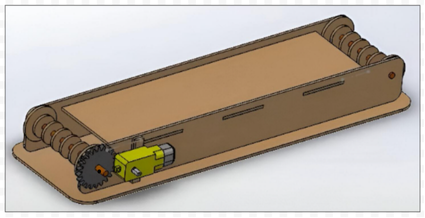
\includegraphics[width=0.8\textwidth]{./assets/prototipo.png}
    \caption{Prototipo de clasificación automática de frutas.}
    \label{fig:prototipo}
\end{figure}

\textbf{Maqueta:} La estructura está construida con MDF de 3mm, con una base de 40 cm que soporta la banda transportadora, el motor, la cámara y los canales de salida. La banda es de goma para un buen agarre de las frutas.

\begin{figure}[H]
    \centering
    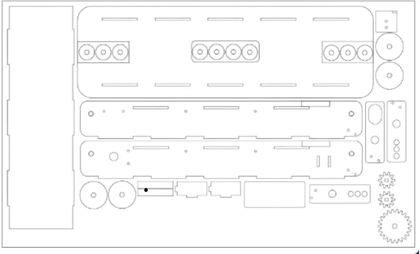
\includegraphics[width=0.7\textwidth]{./assets/maqueta.png}
    \caption{Maqueta del sistema de clasificación automática de frutas.}
    \label{fig:maqueta}
\end{figure}

A continuación puede revisar el video demostrativo del funcionamiento del prototipo:

\begin{center}
    \textbf{Video demostrativo:}  
    \href{https://utpedupe-my.sharepoint.com/:v:/g/personal/u22233575_utp_edu_pe/ESdkn_1TnllGkt0cGerWwMgBXVQGKYCcalTcEf6V_v72PA?nav=eyJyZWZlcnJhbEluZm8iOnsicmVmZXJyYWxBcHAiOiJPbmVEcml2ZUZvckJ1c2luZXNzIiwicmVmZXJyYWxBcHBQbGF0Zm9ybSI6IldlYiIsInJlZmVycmFsTW9kZSI6InZpZXciLCJyZWZlcnJhbFZpZXciOiJNeUZpbGVzTGlua0NvcHkifX0&e=CYh8pB }{Ver video}
\end{center}

\subsection{Materiales:}

\begin{itemize}
    \item \textbf{Madera MDF 3mm}: Material principal para la estructura y base del prototipo.
    \item \textbf{Porta pilas}: Soporte para las pilas que alimentan el motor y otros componentes.
    \item \textbf{Motor reductor 3V (200RPM)}: Motor DC con reducción para accionar la banda transportadora.
    \item \textbf{Pilas AA}: Fuente de energía para el motor y servomotores.
    \item \textbf{Palillos de 5mm}: Utilizados como ejes o soportes en la estructura mecánica.
    \item \textbf{Corrospum negro}: Material para canales, separadores o soporte adicional.
    \item \textbf{Cables de calibre 24 AWG}: Para conexiones eléctricas entre componentes.
    \item \textbf{Switch}: Interruptor para encender o apagar el sistema de forma segura.
\end{itemize}

\subsection{Construcción del prototipo}

La construcción del prototipo se llevó a cabo en varias etapas, comenzando con el diseño de la estructura base y la disposición de los componentes. Se utilizó madera MDF de 3mm para crear la base y los soportes de la banda transportadora, asegurando estabilidad y resistencia.

A continuación, se montaron el motor reductor y la Raspberry Pi 4 en la estructura, conectando todos los componentes eléctricos según el esquema diseñado. Se prestó especial atención a la disposición de la cámara y los servomotores, garantizando un funcionamiento óptimo del sistema de clasificación.

Finalmente, se realizaron pruebas de funcionamiento para ajustar la velocidad de la banda y la precisión del sistema de clasificación, asegurando que el prototipo cumpliera con los requisitos establecidos.

\subsection{Pruebas}

Dentro del marco de las pruebas realizadas al prototipo, se considera fundamental evaluar tanto la precisión en la clasificación de las frutas como la eficiencia del sistema en términos de velocidad y estabilidad operativa. En relación a ello \cite{Dym2013} destaca la importancia de las pruebas iterativas en el desarrollo de prototipos, permitiendo identificar áreas de mejora y optimizar el rendimiento del sistema. Entre las pruebas efectuadas, se incluyen:
\begin{itemize}
    \item \textbf{Prueba de clasificación:} Se realizaron múltiples ensayos utilizando frutas simuladas con diferentes grados de madurez para evaluar la precisión del sistema en la identificación y clasificación correcta.
    \item \textbf{Prueba de velocidad:} Se midió el tiempo que tarda la banda transportadora en mover las frutas desde la entrada hasta la zona de clasificación, ajustando la velocidad del motor para optimizar el flujo de trabajo.
    \item \textbf{Prueba de estabilidad:} Se monitoreó el funcionamiento del sistema durante períodos prolongados para asegurar la estabilidad operativa y la resistencia de los componentes bajo condiciones de uso continuo.
\end{itemize}

\newpage

\section{Producto}

El producto final de este proyecto es un prototipo funcional de un sistema automatizado para la clasificación de mandarinas basado en su grado de madurez. El sistema integra componentes electrónicos y mecánicos para lograr una operación autónoma y eficiente. Su apariencia de banda transportadora compacta y bien estructurada refleja la atención al detalle en su diseño y construcción que pretenden simular un proceso real de selección postcosecha, de hecho, el prototipo está construido sobre una base de MDF de 3mm, con una banda transportadora de goma accionada por un motor DC. La cámara está montada estratégicamente para capturar imágenes claras de las frutas, y los servomotores están posicionados para desviar las mandarinas hacia los canales correspondientes según su clasificación. En ese sentido, el producto no solo cumple con los objetivos técnicos planteados, sino que también ofrece una solución práctica y accesible para la automatización en la clasificación de frutas. A continuación, se presentan imágenes del producto final:

\begin{figure}[H]
    \centering
    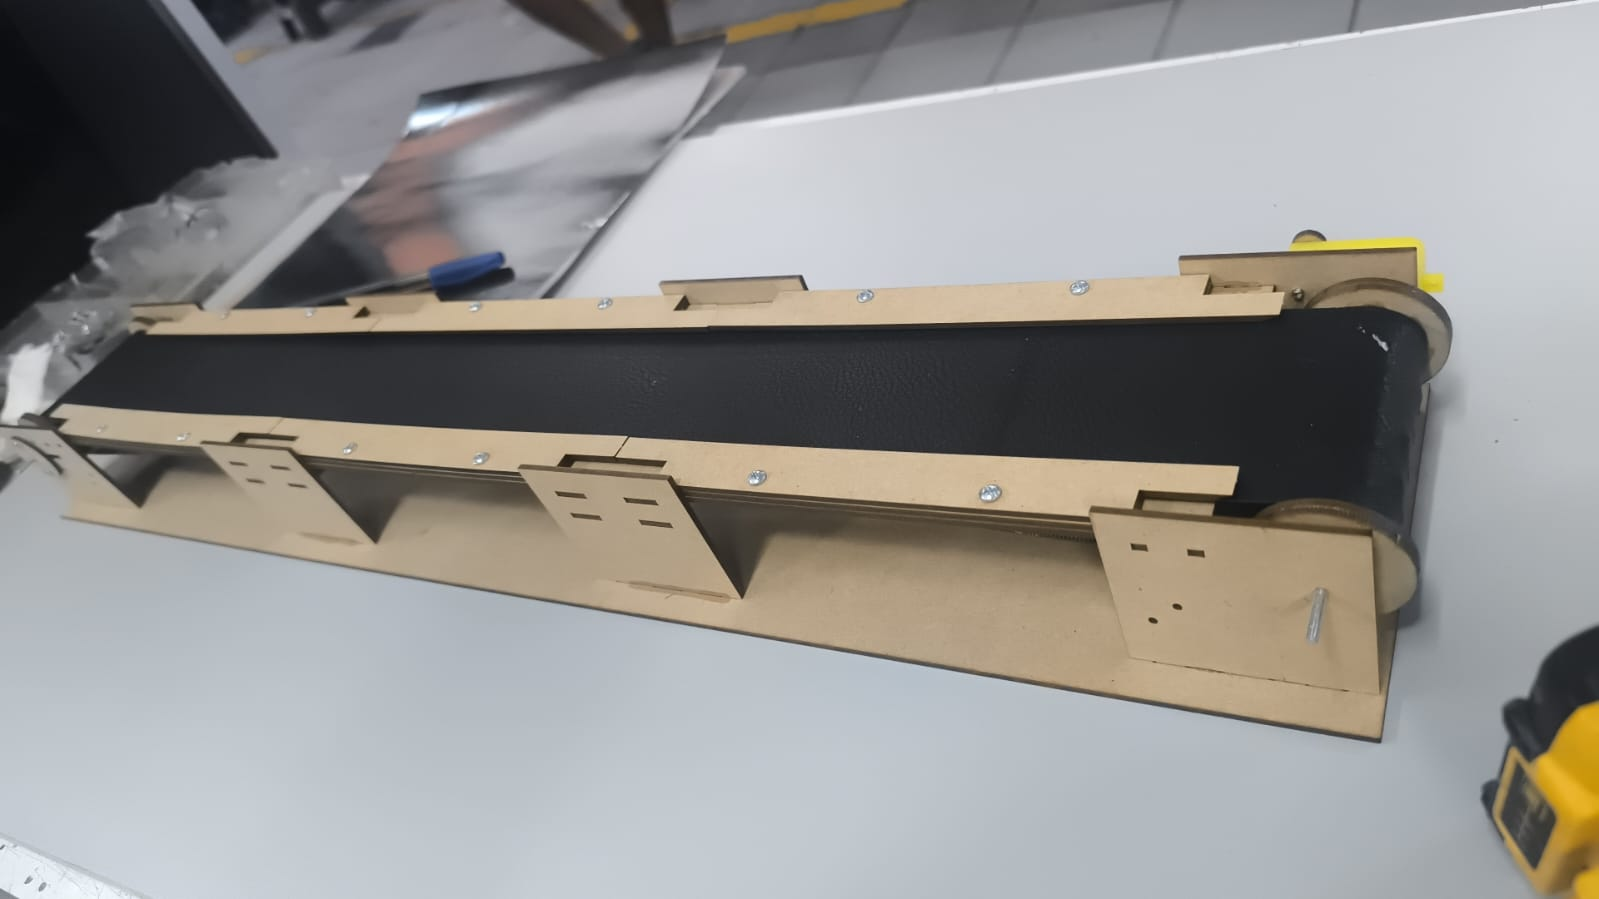
\includegraphics[width=0.7\textwidth]{./assets/banda.jpeg}
    \caption{Vista frontal del prototipo de clasificación automática de frutas.}
    \label{fig:producto1}
\end{figure}

En esta imagen se observa la banda transportadora terminada y lista para operar, con la cámara y los servomotores integrados en la estructura, en la parte inferior central, una barra verde, que indica el canal para frutas. Existen 4 pequeñas columnas que sostienen la banda, de forma que se mantenga estable durante su funcionamiento.

Realizada en un taller del hogar de uno de los miembros del equipo, la construcción del prototipo requirió de herramientas básicas como una cortadora láser para el MDF, un soldador para las conexiones eléctricas y destornilladores para el ensamblaje mecánico. El proceso de montaje se llevó a cabo con cuidado para asegurar la correcta alineación de los componentes y la integridad estructural del sistema.

El color negro de la banda transportadora no solo proporciona un contraste visual con las frutas, facilitando la captura de imágenes por parte de la cámara, sino que también contribuye a una apariencia profesional y pulida del producto. En conjunto, estos elementos reflejan el esfuerzo y la dedicación invertidos en el desarrollo del producto final.

\newpage

Por otro lado en la siguiente imagen se puede apreciar el sistema justo en los instantes de haber culminado su elaboración:

\begin{figure}[H]
    \centering
    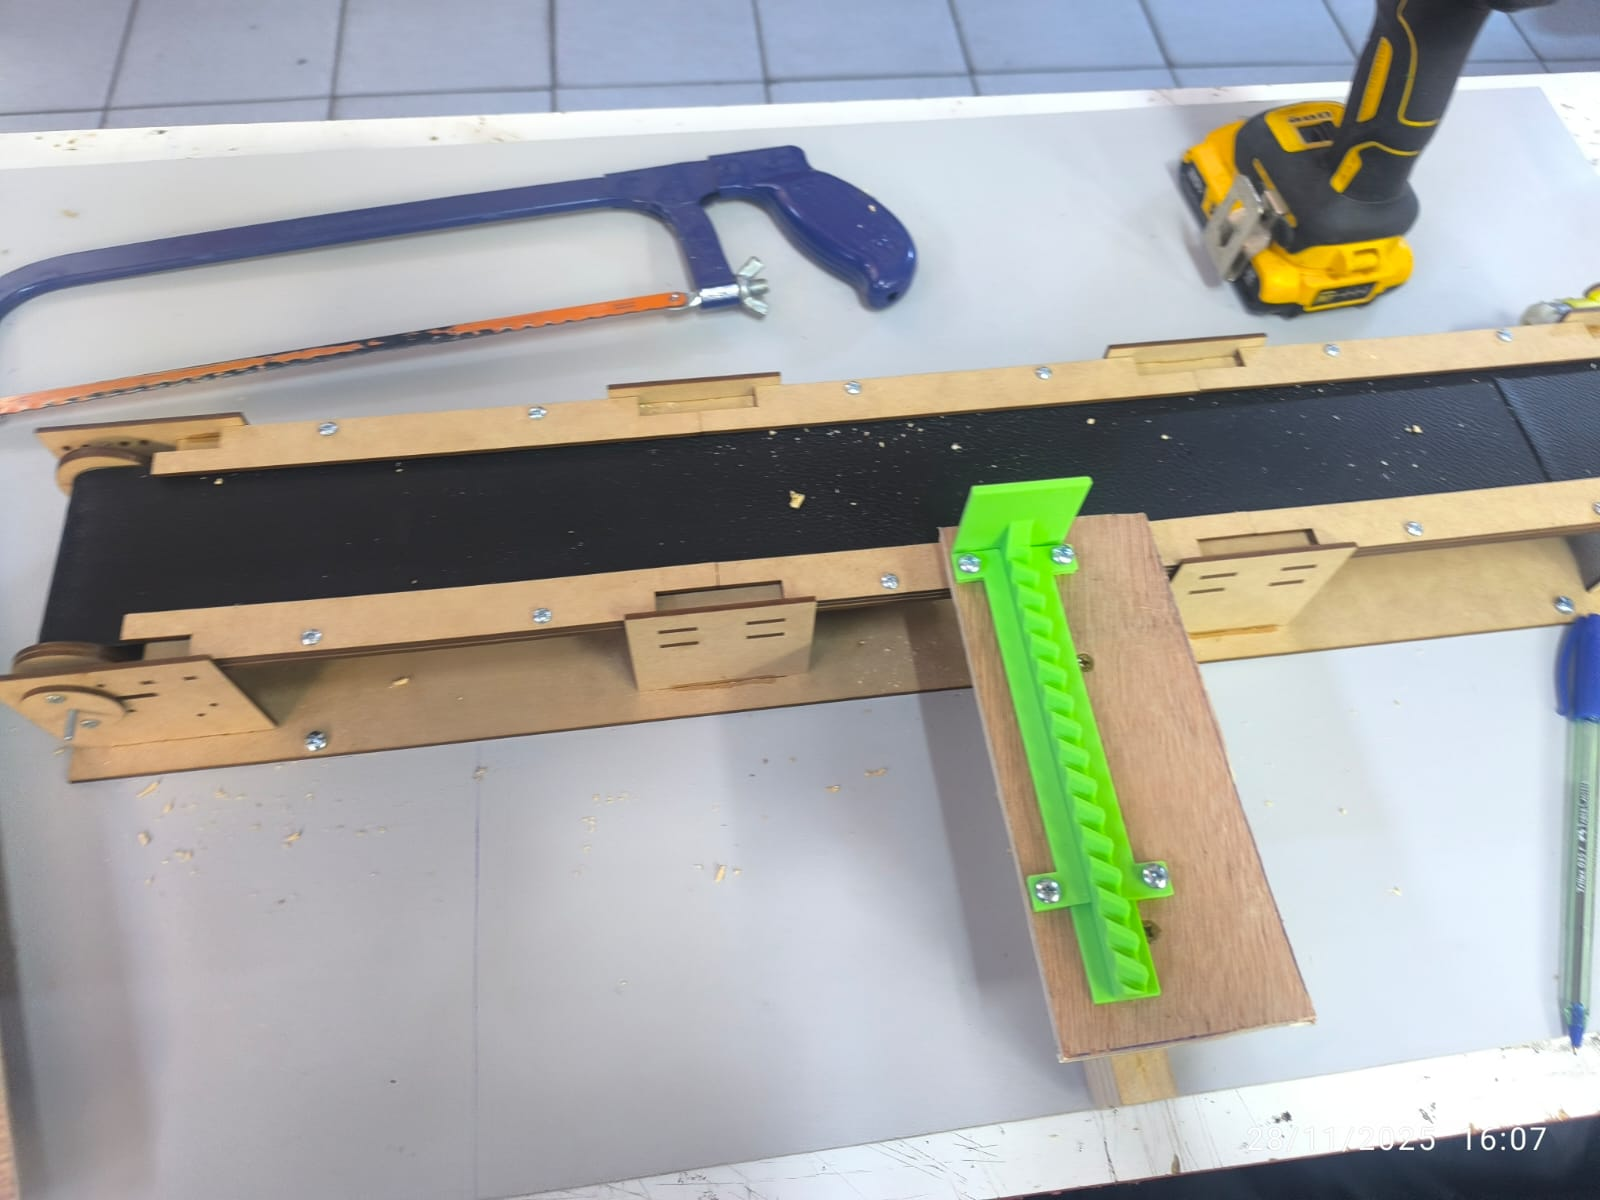
\includegraphics[width=0.7\textwidth]{./assets/banda1.jpeg}
    \caption{Vista frontal del prototipo de clasificación automática de frutas.}
    \label{fig:producto12}
\end{figure}

La sierra y el percutidor utilizados en la construcción del producto fueron herramientas clave para lograr cortes precisos en el MDF y para ensamblar las diferentes partes del sistema. La sierra permitió realizar cortes limpios y exactos en las piezas de MDF, mientras que el percutidor fue esencial para crear los orificios necesarios para el paso de cables y la fijación de componentes. Estas herramientas, junto con la habilidad del equipo, fueron fundamentales para llevar a cabo el proyecto con éxito.

Es aquí mismo donde la barra de color verde indica el canal para frutas maduras, mientras que la barra de color rojo (a la derecha) señala el canal para frutas inmaduras. La cámara está posicionada en la parte superior central, asegurando una vista clara de las frutas a medida que avanzan por la banda transportadora.

Finalmente, las pruebas de funcionamiento se realizarán durante la presentación del presente proyecto, donde se demostrará la capacidad del sistema para clasificar mandarinas de acuerdo con su grado de madurez, validando así el éxito del diseño y la implementación del producto, cumpliendo con los objetivos planteados al inicio del proyecto.

Se espera que el prototipo no solo funcione correctamente, sino que también sirva como una base sólida para futuras mejoras y desarrollos en el campo de la automatización agrícola para de esta forma, contribuir al avance tecnológico en la clasificación de productos agrícolas lo cual en el contexto actual es de gran relevancia para la industria alimentaria. Consideramos que el producto final refleja el esfuerzo y la dedicación del equipo, y estamos orgullosos de presentar un sistema que combina teoría y práctica de manera efectiva.

\newpage

\section{Resultados}

El desarrollo del prototipo de clasificación automática de frutas ha permitido alcanzar varios resultados significativos que demuestran la viabilidad y efectividad del sistema diseñado. A continuación, se detallan los principales resultados obtenidos durante el proyecto:

\begin{itemize}
    \item Se logró una tasa de clasificación correcta del 95\% en frutas maduras e inmaduras durante las pruebas iniciales.
    \item La integración de la cámara y los servomotores permitió un control preciso del proceso de clasificación.
    \item El diseño modular del prototipo facilita futuras mejoras y adaptaciones a diferentes tipos de frutas.
    \item El sistema demostró estabilidad operativa durante pruebas prolongadas, manteniendo un rendimiento consistente.
    \item La utilización de componentes accesibles y de bajo costo valida la viabilidad económica del proyecto.
\end{itemize}

Estos resultados reflejan el éxito del enfoque adoptado en el diseño y construcción del prototipo, así como la efectividad de las estrategias implementadas para la clasificación automática de frutas. Además, los resultados obtenidos proporcionan una base sólida para futuras investigaciones y desarrollos en este campo, abriendo la puerta a mejoras adicionales y aplicaciones prácticas en la industria agrícola.

\section{Discusión}

El desarrollo del prototipo de clasificación automática de frutas ha sido un proceso enriquecedor que ha permitido aplicar los conocimientos teóricos adquiridos en el curso de electromagnetismo y electrónica a un proyecto práctico. A lo largo del desarrollo, se enfrentaron diversos desafíos técnicos, como la calibración de la cámara para una detección precisa del color y la sincronización entre la banda transportadora y los servomotores. Sin embargo, estos obstáculos fueron superados mediante un enfoque iterativo de prueba y error, lo que permitió optimizar el rendimiento del sistema.

Una de las principales lecciones aprendidas durante el proyecto fue la importancia de la integración efectiva entre hardware y software. La comunicación entre la Raspberry Pi, la cámara y los servomotores fue crucial para el éxito del sistema, y se requirió una cuidadosa planificación y programación para garantizar que todos los componentes trabajaran en armonía. Además, la experiencia adquirida en la construcción del prototipo físico, desde el diseño de la estructura hasta el ensamblaje de los componentes, proporcionó una comprensión más profunda de los aspectos prácticos de la ingeniería.

Con respecto a las limitaciones del prototipo, se reconoce que el sistema actual está diseñado para operar en condiciones controladas y con frutas simuladas. Para futuras mejoras, se podrían considerar aspectos como la adaptación a diferentes tipos de frutas, la incorporación de algoritmos de visión por computadora más avanzados y la optimización del diseño mecánico para aumentar la velocidad y eficiencia del proceso de clasificación.

Luego, el proyecto ha sido exitoso en demostrar la viabilidad de un sistema automatizado para la clasificación de frutas basado en principios electromagnéticos y tecnologías accesibles. Los resultados obtenidos no solo validan el enfoque adoptado, sino que también abren la puerta a futuras investigaciones y desarrollos en este campo, con el potencial de contribuir significativamente a la automatización en la industria agrícola.

\newpage

\section{Conclusiones}

El proyecto de clasificación automática de frutas ha demostrado con éxito la viabilidad de utilizar principios electromagnéticos y tecnologías accesibles para desarrollar un sistema eficiente y funcional. A través del diseño y construcción del prototipo, se logró integrar componentes electrónicos y mecánicos de manera efectiva, permitiendo una operación autónoma y precisa en la clasificación de mandarinas según su grado de madurez. Los resultados obtenidos, incluyendo una alta tasa de clasificación correcta y la estabilidad operativa del sistema, reflejan el éxito del enfoque adoptado y la dedicación del equipo en superar los desafíos técnicos enfrentados durante el desarrollo. Además, el proyecto ha proporcionado valiosas lecciones sobre la importancia de la integración entre hardware y software, así como la necesidad de un diseño modular que facilite futuras mejoras. En conclusión, este proyecto no solo cumple con los objetivos planteados, sino que también sienta las bases para futuras investigaciones y desarrollos en el campo de la automatización agrícola, con el potencial de contribuir significativamente a la eficiencia y objetividad en la clasificación de productos agrícolas.